\chapter*{Conclusion}
\addcontentsline{toc}{chapter}{Conclusion}
\label{chapter:summary}

\section*{List of publications}
\addcontentsline{toc}{section}{List of publications}

\subsection*{Publications in international scientific journals}
\addcontentsline{toc}{subsection}{Publications in international scientific journals}

A list of publications related to the dissertation follows. The listed articles have been published without exception in international scientific journals. [1] is an early version of the Introduction as well Chapter~\ref{chapter-openbiodiv} and contains work towards Objective 1 (Architecture). [2, 3, 5, 6, 7] are not a part of the text of the dissertation but can be considered work towards Objective 5 (Workflows). [4] is also a publication towards Objective 5 (Workflows) and a version of it served as the bases for Chapter~\ref{chapter-case-study}. [7] is published in the peer-reviewed journal ZooKeys with impact factor 1.031 (early 2018). [8] is the most important publication under this dissertation and was published in the high-impact Journal of Biomedical Semantics with impact factor 2.413 (early 2018). [8] makes up the content of Chapter~\ref{chapter-ontology} and is the main body of work fulfilling Objective 2 (Ontology). It was a featured article on the home-page of JBS (Fig.~\ref{fig:jbs-featured}). Chapter~\ref{chapter-lod} and Chapter~\ref{chapter-rdf4r} that form Objectives 3, 4, respectively are currently being prepared as manuscripts in international journals. Furthermore, the software library RDF4R described in Chapter~\ref{chapter-rdf4r} is being submitted to the open source repository ROpenSci.

The total number of citations that have been accumulated excluding self-citations (cross-citations) is at least 19. The total number of citations that have been accumulated including cross-citations and citations of work outside of the scope of the dissertation is at least 46 (Google Scholar).

\begingroup
\newcounter{count}
\setcounter{count}{99}
\defcounter{maxnames}{\value{count}}%

\begin{enumerate}
\item \longfullcite{senderov_open_2016} (at least 3 unique citations)
\item \longfullcite{sarah_faulwetter_emodnet_2016}
\item \longfullcite{cardoso_species_2016} (at least 5 unique citations)
\item \longfullcite{senderov_online_2016} (at least 1 unique citation)
\item \longfullcite{penev_strategies_2017} (at least 6 unique citations)
\item \longfullcite{penev_arpha-biodiv:_2017} (at least 1 unique citations)
\item \longfullcite{arriaga-varela_review_2017} 
\item \longfullcite{senderov_openbiodiv-o:_2018} (at least 3 unique citations)
\end{enumerate}
\endgroup

\begin{figure}
\centering
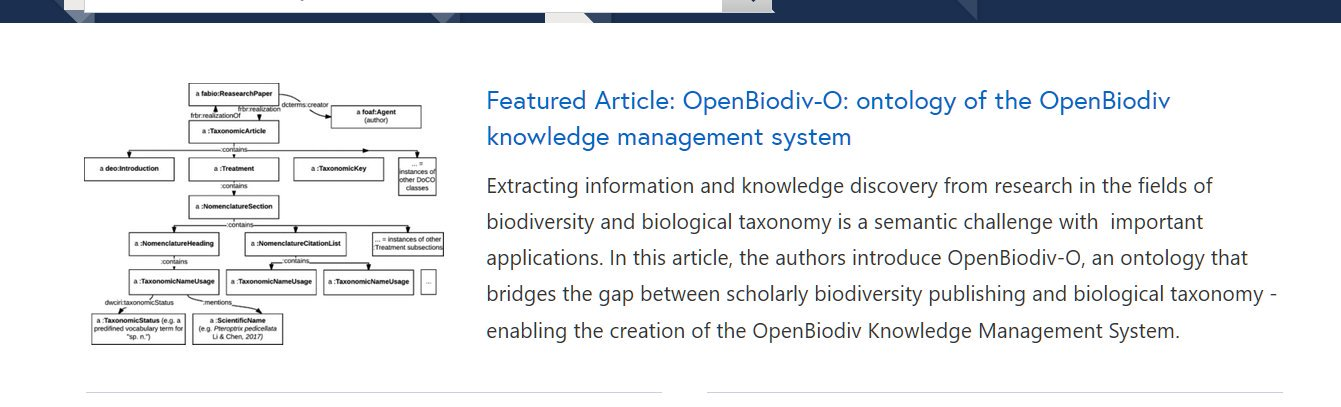
\includegraphics[width=\textwidth]{Figures/JBS-featured.jpg}
\decoRule
\caption{The OpenBiodiv-O article is featured on the main webpage of the Journal of Biomedical Semantics..}
\label{fig:jbs-featured}
\end{figure}

\section*{Апробация на резултатите}
\addcontentsline{toc}{section}{Апробация на резултатите}

\subsection*{Доклади пред научен семинар на ПНЗ}
\addcontentsline{toc}{subsection}{Доклади пред научен семинар на ПНЗ}

\begin{enumerate}
    \item Доклад пред научен семинар на ИБЕИ на БАН на 26.10.2015 г. (“Публикуване, визуализация и разпространение на първични и геномни данни за биологичното разнообразие на основата на открита система за управление на информацията”).
    \item Доклад пред научен семинар в ИИКТ на БАН на 31.03.2016 г. (Open Biodiversity Knowledge Management System)
    \item Dоклад пред научен семинар на ИИКТ на БАН за 23.03.2018 г. (OpenBiodiv: a knowledge-based system of biodiversity information)
\end{enumerate}

\subsection*{Доклади пред научно мероприятие в чужбина или пред международно научно мероприятие у нас}
\addcontentsline{toc}{subsection}{Доклади пред научно мероприятие в чужбина или пред международно научно мероприятие у нас}

\begin{enumerate}
    \item Доклад пред международния симпозиум EU BON в София на 23.03.2016 г. (The Data Publishing Toolkit at EU BON: Automated creation of data papers, data and text integrated publishing via the ARPHA Publishing Platform.)
    \item Доклад по време на работната среща на BIG4 в Хавраники, Чехия на 03.06.2016 г. (Project Progress Report (OBKMS))
    \item Доклад по време на работната среща на BIG4 в Хавраники, Чехия на 03.06.2016 г. (Modern Methods of Systematic Research and the BOLD Algorithm)
    \item Уеб-базиран доклад (уебинар) пред международна аудитория в рамките на семинар на iDigBio на 16.07.2016 г. (Online direct import of specimen records from iDigBio instrastructure into taxonomic manuscripts)
    \item Доклад по време на работната среща на BIG4 в Копенхаген на 14.10.2016 г. (Midterm Progress Report)
    \item Доклад на международия симпозиум TDWG 2016 в Санта Клара де Сан Карлос от 5. до 9.12.2016 г. (Streamlining the Flow of Taxon Occurrence Data Between a Manuscript and Biological Databases)
    \item Доклад на международия симпозиум TDWG 2016 в Санта Клара де Сан Карлос от 5. до 9.12.2016 г. (The Open Biodiversity Knowledge Management System: A Semantic Suite Running on top of the Biodiversity Knowledge Graph)
    \item Доклад на международия симпозиум TDWG 2016 в Санта Клара де Сан Карлос от 5. до 9.12.2016 г. (Demonstrating the Prototype of the Open Biodiversity Knowledge Management System)
    \item Доклад на международия симпозиум TDWG 2016 в Санта Клара де Сан Карлос от 5. до 9.12.2016 г. (Creation of Data Paper Manuscripts from Ecological Metadata Language (EML))
    \item Уеб-базиран доклад пред междуродния семинар на работната група по семантични технология към Университета Вандербилт (Тенеси, САЩ) на 20.02.2017 г. (Open Biodiversity Knowledge Management System)
    \item Доклад на европейската конференция на биосистематиците, BioSyst.eu 2016 на 15.08.2017 г. (The OpenBiodiv Knowledge System: The Future of Access to Biodiversity Knowledge)
    \item Доклад на международия симпозиум TDWG 2017 в Отава, Канада от 1. до 6.10.2017 г. (OpenBiodiv Computer Demo: an Implementation of a Semantic System Running on top of the Biodiversity Knowledge Graph)
    \item Доклад на международия симпозиум TDWG 2017 в Отава, Канада от 1. до 6.10.2017 г. (OpenBiodiv: an Implementaion of a Semantic System Running on top of the Biodiversity Knowledge Graph)
    \item Постер на международия симпозиум TDWG 2017 в Отава, Канада от 1. до 6.10.2017 г. (OpenBiodiv: an Implementaion of a Semantic System Running on top of the Biodiversity Knowledge Graph)
    \item Доклад по време на работната среща на BIG4 в Ла Палма, Испания от 30. окт. до 3 ноем. 2017 г. (Midterm Progress Report)
    \item Доклад пред научен семинар на групата по биоинформатика (група Ронкуист) в Кралския природо-научен музей в Стокхолм на 29.11.2017 г.
\end{enumerate}

\section*{Main scientific and applied contributions}
\addcontentsline{toc}{section}{Main scientific and applied contributions}


In the course of the investigative effort, all six objectives have been achieved and the results have been published in international journals and have been presented at major conferences in Bulgaria and abroad. We have made several significant contributions that we would like summarize in this section. 

\paragraph{Contribution 1.} The first key contribution of the thesis is the creation of the software architecture of the OpenBiodiv system outlined in Chapter~\ref{chapter-openbiodiv} and \cite{senderov_open_2016}. This contribution fulfills Objective 1.

\paragraph{Contribution 2} The second key contribution of the thesis is the creation of a domain conceptualization and a formal ontology OpenBiodiv-O enabling the linking of biodiversity knowledge on the basis of scholarly publications. OpenBiodiv-O, serves as the basis of the linked open data OpenBiodiv-LOD. By developing an ontology focusing on biological taxonomy, our intent is to provide an ontology that fills in the gaps between ontologies for biodiversity resources such as Darwin-SW and semantic publishing ontologies such as the ontologies comprising the SPAR Ontologies. Moreover, we take the view that it is advantageous to model the taxonomic process itself rather than any particular state of knowledge. This contribution has been described in Chapter~\ref{chapter-ontology} and in \cite{senderov_openbiodiv-o:_2018} and fulfills Objective 2. Its source code can be viewed under \href{https://github.com/vsenderov/openbiodiv-o}{github.com/vsenderov/openbiodiv-o}

\paragraph{Contribution 3.} The third key contribution of the thesis has been the creation of a linked open dataset, OpenBiodiv-LOD, consisting of a transformation to RDF-triples and integration in a single store of information from three major repositories of biodiversity data: the XML sources of biological journals published by Pensoft Publishers, the XML sources of treatments freed by Plazi, and a CSV dump of GBIF's taxonomic backbone. OpenBiodiv-LOD is available under \href{http://graph.openbiodiv.net}{\url{graph.openbiodiv.net}} and has been described in Chapter~\ref{chapter-lod}. This contribution fulfills Objective 3.

\paragraph{Contribution 4.} In order to  create the linked open data, a software package for the R programming environment, RDF4R, was developed. RDF4R enables the manipulation of RDF data within R and facilities the transformation of scientific publications from a semi-structured XML format to structured semantic RDF. This contribution has been discussed in Chapter~\ref{chapter-rdf4r} and fulfills Objective 4. The package is available online as free software under \href{http://github.com/vsenderov/rdf4r}{\url{github.com/vsenderov/rdf4r}}. Furthermore, additional source code (unoptimized) describing XML schemas of Pensoft and Plazi and working in tandem with RDF4R to convert XML to RDF can be found under \href{http://github.com/vsenderov/ropenbio}{\url{github.com/vsenderov/ropenbio}}.

\paragraph{Contribution 5.} The mechanisms to convert semi-structured XML into RDF-triples are complemented by workflows enabling the enrichment of the XML sources of Pensoft journals by data automatically imported from the major international biodiversity data repositories---BOLD, GBIF, iDigBio, as well as PlutoF. Furthermore, it is now possible, thanks to this dissertation effort to automatically create manuscripts from metadata encoded in the Ecological Metadata Language (EML). The discussion of these automated workflows---automatic data paper generation and automatic occurrence record import---is carried out in Chapter~\ref{chapter-case-study}. It fulfills Objective 5.

\paragraph{Contribution 6.} To complement the creation of OpenBiodiv-LOD, we have developed a web-site running on top of the knowledge graph \href{http://openbiodiv.net}{openbiodiv.net}, containing a semantic search engine and apps. The website is discussed in Chapter~\ref{chapter-openbiodiv} and fulfills Objective 6.

\section*{Декларация за оригиналност}
\addcontentsline{toc}{section}{Декларация за оригиналност}

Декларирам, че настоящата дисертация съдържа оригинални резултати, получени 
при проведени от мен научни изследвания, с подкрепата и съдействието на научния ми ръководител проф. Любомир Пенев и Издаделство Пенсофт, както и научния ми консултант доц. Кирил Симов и ИИКТ.  Резултатите,  които  са  получени,  описани  и/или  публикувани  от  други учени, са надлежно и подробно цитирани в библиографията.

Настоящата дисертация не е прилагана за придобиване на научна степен в друго 
висше училище, университет или научен институт.

Виктор Сендеров

%----------------------------------------------------------------------------------------
%	ACKNOWLEDGEMENTS
%----------------------------------------------------------------------------------------

\begin{acknowledgements}
\addchaptertocentry{\acknowledgementname} % Add the acknowledgements to the table of contents

This research has been financed through the European Union’s Horizon 2020 research and innovation program under the Marie Sklodowska-Curie grant agreement No. 642241. My deep gratitude goes to the European Commission for enabling this wonderful opportunity!

\vspace{5mm}

I thank Prof. Lyubomir Penev and Prof. Kiril Simov for the valuable supervision. I also thank the staff and developers at Pensoft Publishers for the support in creating the platform and its popularization; in particular Prof. Pavel Stoev, Teodor Georgiev, Georgi Zhelezov, Iliyana Kuzmova, and Iva Kostadinova.

\vspace{5mm}

I thank my colleagues from the Bulgarian Academy of Sciences (Institutes for Information and Communication Technologies and for Biodiviversity and Ecosystems Research) for their friendship and advice; in particular Prof. Galya Angelova, Prof. Boyko Georgiev, and Prof. Snejana Grozeva.

\vspace{5mm}

I thank my colleagues at the BIG4 training network for the feedback, friendship, and support. In particular Prof. Alexey Solovdnikov, but there are too many more names to mention.

\vspace{5mm}

I thank my international collaborators for their ideas, reviews, and collaboration on papers. In particular Prof. Nico Franz (Arizona State University), Dr. Daniel Mietchen (National Institutes of Health), Dr.  Éamonn Ó Tuama (formerly at GBIF), and Prof. Bob Morris (emeritus UMASS).

\vspace{5mm}

I also thank everyone at Plazi for the co-ownership of the vision of the project; in particular, Dr. Donat Agosti, Terry Catapano, and Dr. Guido Sautter.

\vspace{5mm}

Last but not least, I would like to acknowledge Ontotext for building the GraphDB database and providing excellent support.



\end{acknowledgements}